\chapter{Enterprise Edition: Domains, Governance and the SDK}
\label{ch:enterprise}

Version 0.2 takes \algolang\ from the classroom to the organisation. A university, hospital, bank or ministry rarely needs one multi-agent program. It needs dozens of them across many departments, all under the same rules, all auditable, and usable by staff who will never write code. This chapter describes the six additions that make that possible:

\begin{enumerate}
\item \textbf{Modules}: \kw{use} imports for building large systems from small ones.
\item \textbf{Org policy}: one \file{algo.config.json} that governs every program.
\item \textbf{120 domain packs} covering 20 sectors.
\item \textbf{Governance}: a hash-chained audit log, a human review queue and reports.
\item \textbf{Executable tools and scale}: plugin tools, a live tool-use loop, batch runs and a global concurrency limit.
\item \textbf{One SDK, three modes}: command line, graphical Studio and the new Prompt-based UI.
\end{enumerate}

\section{Modules}

A file can import agents from another file, or from a domain pack. Imported agents are used through their alias, so names never clash.

\begin{algo}[title=examples/enterprise/claims\_pipeline.algo]
use "common/intake.algo" as intake
use pack insurance.fraud_screening as fraud
use pack insurance.claims_triage as claims

policy {
    budget tokens 8000
    forbid religion, caste
}

flow main(claim: text) {
    c     = intake.Normaliser(claim)
    views = par { fraud.PatternAnalyst(c), fraud.DocumentExaminer(c), fraud.Adjuster(c) }
    risk  = fraud.FraudPanel(views)
    level = claims.Complexity(c)
    if risk > 0.7 {
        note = fraud.Referral(views, risk)
        emit c, risk, note
    }
    route = claims.Routing(c, level)
    emit c, risk, route
}
\end{algo}

\begin{itemize}
\item \code{use "path.algo" as x} imports a file. The path is relative to the importing file.
\item \code{use pack sector.name as x} imports a domain pack. Packs are found in \file{packs/} and in any folder listed in the \code{ALGO\_PACKS} environment variable.
\item A top-level \kw{policy} block is the file's default. Every agent in the file inherits it, and its own policy can only make it stricter.
\item Errors inside an imported file are reported with that file's name. Circular imports are rejected.
\end{itemize}

\section{Organisation policy}

\code{algo init} writes \file{algo.config.json}. The runtime looks for it in the current folder and its parents. Its rules are merged into the policy of \emph{every} agent in \emph{every} program, and \textbf{the stricter rule always wins}:

\begin{itemize}
\item forbidden attributes are joined together;
\item budgets take the smaller value;
\item human-review thresholds take the higher value.
\end{itemize}

No program can relax the organisation's rules.

\begin{center}
\small
\begin{tabularx}{\linewidth}{@{}L{3.6cm}Y@{}}
\toprule
\thead{Key} & \thead{Effect}\\
\goldrule
\code{forbid} & Attributes no agent may take as input, checked at compile time (\errcode{E108}) and at run time\\
\code{max\_budget\_tokens} & Upper limit on any agent's \code{budget tokens}\\
\code{min\_human\_below} & Every agent is escalated to a human below this confidence\\
\code{allowed\_tools} & Only these tools may be declared (\code{null} allows all)\\
\code{max\_concurrency} & Global limit on simultaneous model calls, shared by all threads and batch workers\\
\code{max\_run\_tokens} & Token cap for one complete run\\
\code{cache} & Reuse identical answers from a SQLite cache at zero tokens\\
\code{models}, \code{tools}, \code{plugins} & Model aliases, tool settings, Python files that register company tools\\
\bottomrule
\end{tabularx}
\end{center}

\section{The domain library: 120 packs in 20 sectors}

Each pack is an ordinary \file{.algo} file in \file{packs/<sector>/}. Every pack passes the compiler and runs offline. Packs follow one of four patterns from Chapter~\ref{ch:patterns}:

\begin{description}
\item[pipe] a chain of specialists;
\item[fan] parallel specialists and a synthesiser;
\item[committee] parallel reviewers and a scoring panel;
\item[router] a classifier that sends work to the right desk.
\end{description}

Policies are set by risk level. High-risk packs escalate below 0.90 confidence, medium-risk below 0.80 and low-risk below 0.70. Healthcare and pharma packs also forbid protected attributes.

\begin{center}
\small
\begin{tabularx}{\linewidth}{@{}YYYY@{}}
\toprule
\multicolumn{4}{@{}l}{\thead{Sectors (6 packs each)}}\\
\goldrule
Healthcare & Pharma \& Life Sciences & Banking & Insurance\\
Capital Markets & Education & Research \& Academia & Government\\
Legal \& Compliance & HR \& Workforce & Manufacturing & Supply Chain\\
Retail \& E-commerce & Telecom \& IT Ops & Cybersecurity & Energy \& Utilities\\
Agriculture & Media \& Marketing & Real Estate & Hospitality \& Travel\\
\bottomrule
\end{tabularx}
\end{center}

\begin{terminal}
$ algo domains "our servers are down and customers cannot log in"
  0.49  itops.incident_triage      IT incident triage
  0.35  itops.log_anomaly          Log anomaly detection
  0.33  itops.postmortem           Incident postmortem writer
$ algo run pack:itops.incident_triage --arg "incident=Login API returns 500"
$ algo pack itops.incident_triage --copy      # save an editable copy
\end{terminal}

Search works offline. It uses TF-IDF over each pack's title, description, agents and sector, with a synonym table and sector hints, so \emph{``citizen complaint about water''} finds the government grievance pack. New domains are added as one line in \file{tools/make\_packs.py}.

\section{Governance}

\paragraph{Hash-chained audit log.} Every agent call is written to \file{runs/<program>.audit.jsonl}. Each record stores the SHA-256 hash of the previous record (\code{prev}) and its own hash (\code{hash}). Changing, inserting or deleting any line breaks the chain. \code{algo audit verify} reports the first bad line. Concurrent writers are serialised, so the chain stays valid under batch load.

\paragraph{Human review queue.} A result below its confidence threshold is \emph{escalated}:
\begin{itemize}
\item it is recorded with status \code{escalated};
\item it is added to an event-sourced queue (\file{runs/review\_queue.jsonl});
\item it is decided later by a named reviewer with \code{algo review approve ID --reviewer NAME}, in the Studio's Governance tab, or with \code{al.review.approve(...)}.
\end{itemize}
Every decision is itself an audit event.

\paragraph{Reports.} \code{algo report} totals calls, tokens, escalations, blocks, cache hits and average confidence for each program and each agent, and checks every chain.

\section{Executable tools and scale}

Tools are real Python functions. The built-in tools are:
\begin{itemize}
\item \code{calc.eval}: safe arithmetic;
\item \code{file.read}: restricted to the project folder;
\item \code{kb.search}: searches \file{kb/}.
\end{itemize}

A company adds its own tools in a plugin file:

\begin{pycode}
import algoruntime as rt

@rt.register_tool("company.directory", "Look up which team owns a topic")
def directory(query):
    return lookup_in_hr_system(query)
\end{pycode}

An agent can call a tool only if it declares it with \kw{uses}, and only if the org config allows it. In live mode the runtime runs Claude's tool-use loop (up to five rounds) and refuses any tool the agent did not declare.

\code{algo batch program.algo --input data.csv --workers 16} runs a program once per CSV row and writes a results CSV. In testing, 200 insurance claims ran in 0.6\,s offline, with the audit chain intact. Live model calls stay within \code{max\_concurrency}.

\section{One SDK, three modes}

\code{import algolang} is the public Python SDK. The command line, Studio and Prompt UI all call it, so a program behaves identically in each.

\begin{pycode}
import algolang as al

al.configure(forbid=["salary", "caste"], min_human_below=0.75)
best = al.domains.search("triage insurance claims")[0]
prog = al.pack(best["id"])                      # or al.load("x.algo"), al.compile(src)
r = prog.run(claim="Rear-end collision in Pune")
print(r.status, r.values, r.stats, len(r.escalated))

results = prog.run_batch(rows, workers=16)      # list of RunResult
plan = al.compose("screen this CV fairly")      # prompt -> best pack + program
al.review.pending(); al.review.approve(item_id, reviewer="Dr. S")
al.audit.verify("runs/claims_triage.audit.jsonl")
\end{pycode}

\subsection{Mode 1: command line}

\begin{center}
\small
\begin{tabularx}{\linewidth}{@{}L{5.6cm}Y@{}}
\toprule
\thead{Command} & \thead{Purpose}\\
\goldrule
\code{algo init acme} & New project: config, plugin tool, knowledge base, sample program and data\\
\code{algo domains [words] [--sector S]} & Search the domain library\\
\code{algo pack ID [--copy]} & Show or copy a pack\\
\code{algo run pack:ID --arg ...} & Run a pack directly\\
\code{algo batch FILE --input CSV} & Parallel batch run\\
\code{algo review [approve|reject ID]} & Human review queue\\
\code{algo audit verify [path]} & Tamper check\\
\code{algo report [--json]} & Usage and governance summary\\
\code{algo chat} & Prompt mode in the terminal\\
\bottomrule
\end{tabularx}
\end{center}

\subsection{Mode 2: graphical Studio}

Studio (Chapter~\ref{ch:modes}) gains three tabs:
\begin{description}
\item[Domains] Sector chips, plain-English search, and pack cards with \emph{Open in editor} and \emph{Use in my program}. The latter inserts a \kw{use pack} line.
\item[Batch] Upload or paste a CSV, run it, and download the results.
\item[Governance] Usage tiles, a per-program table, the review queue with Approve and Reject, and the active org policy.
\end{description}

\begin{figure}[ht]
\centering
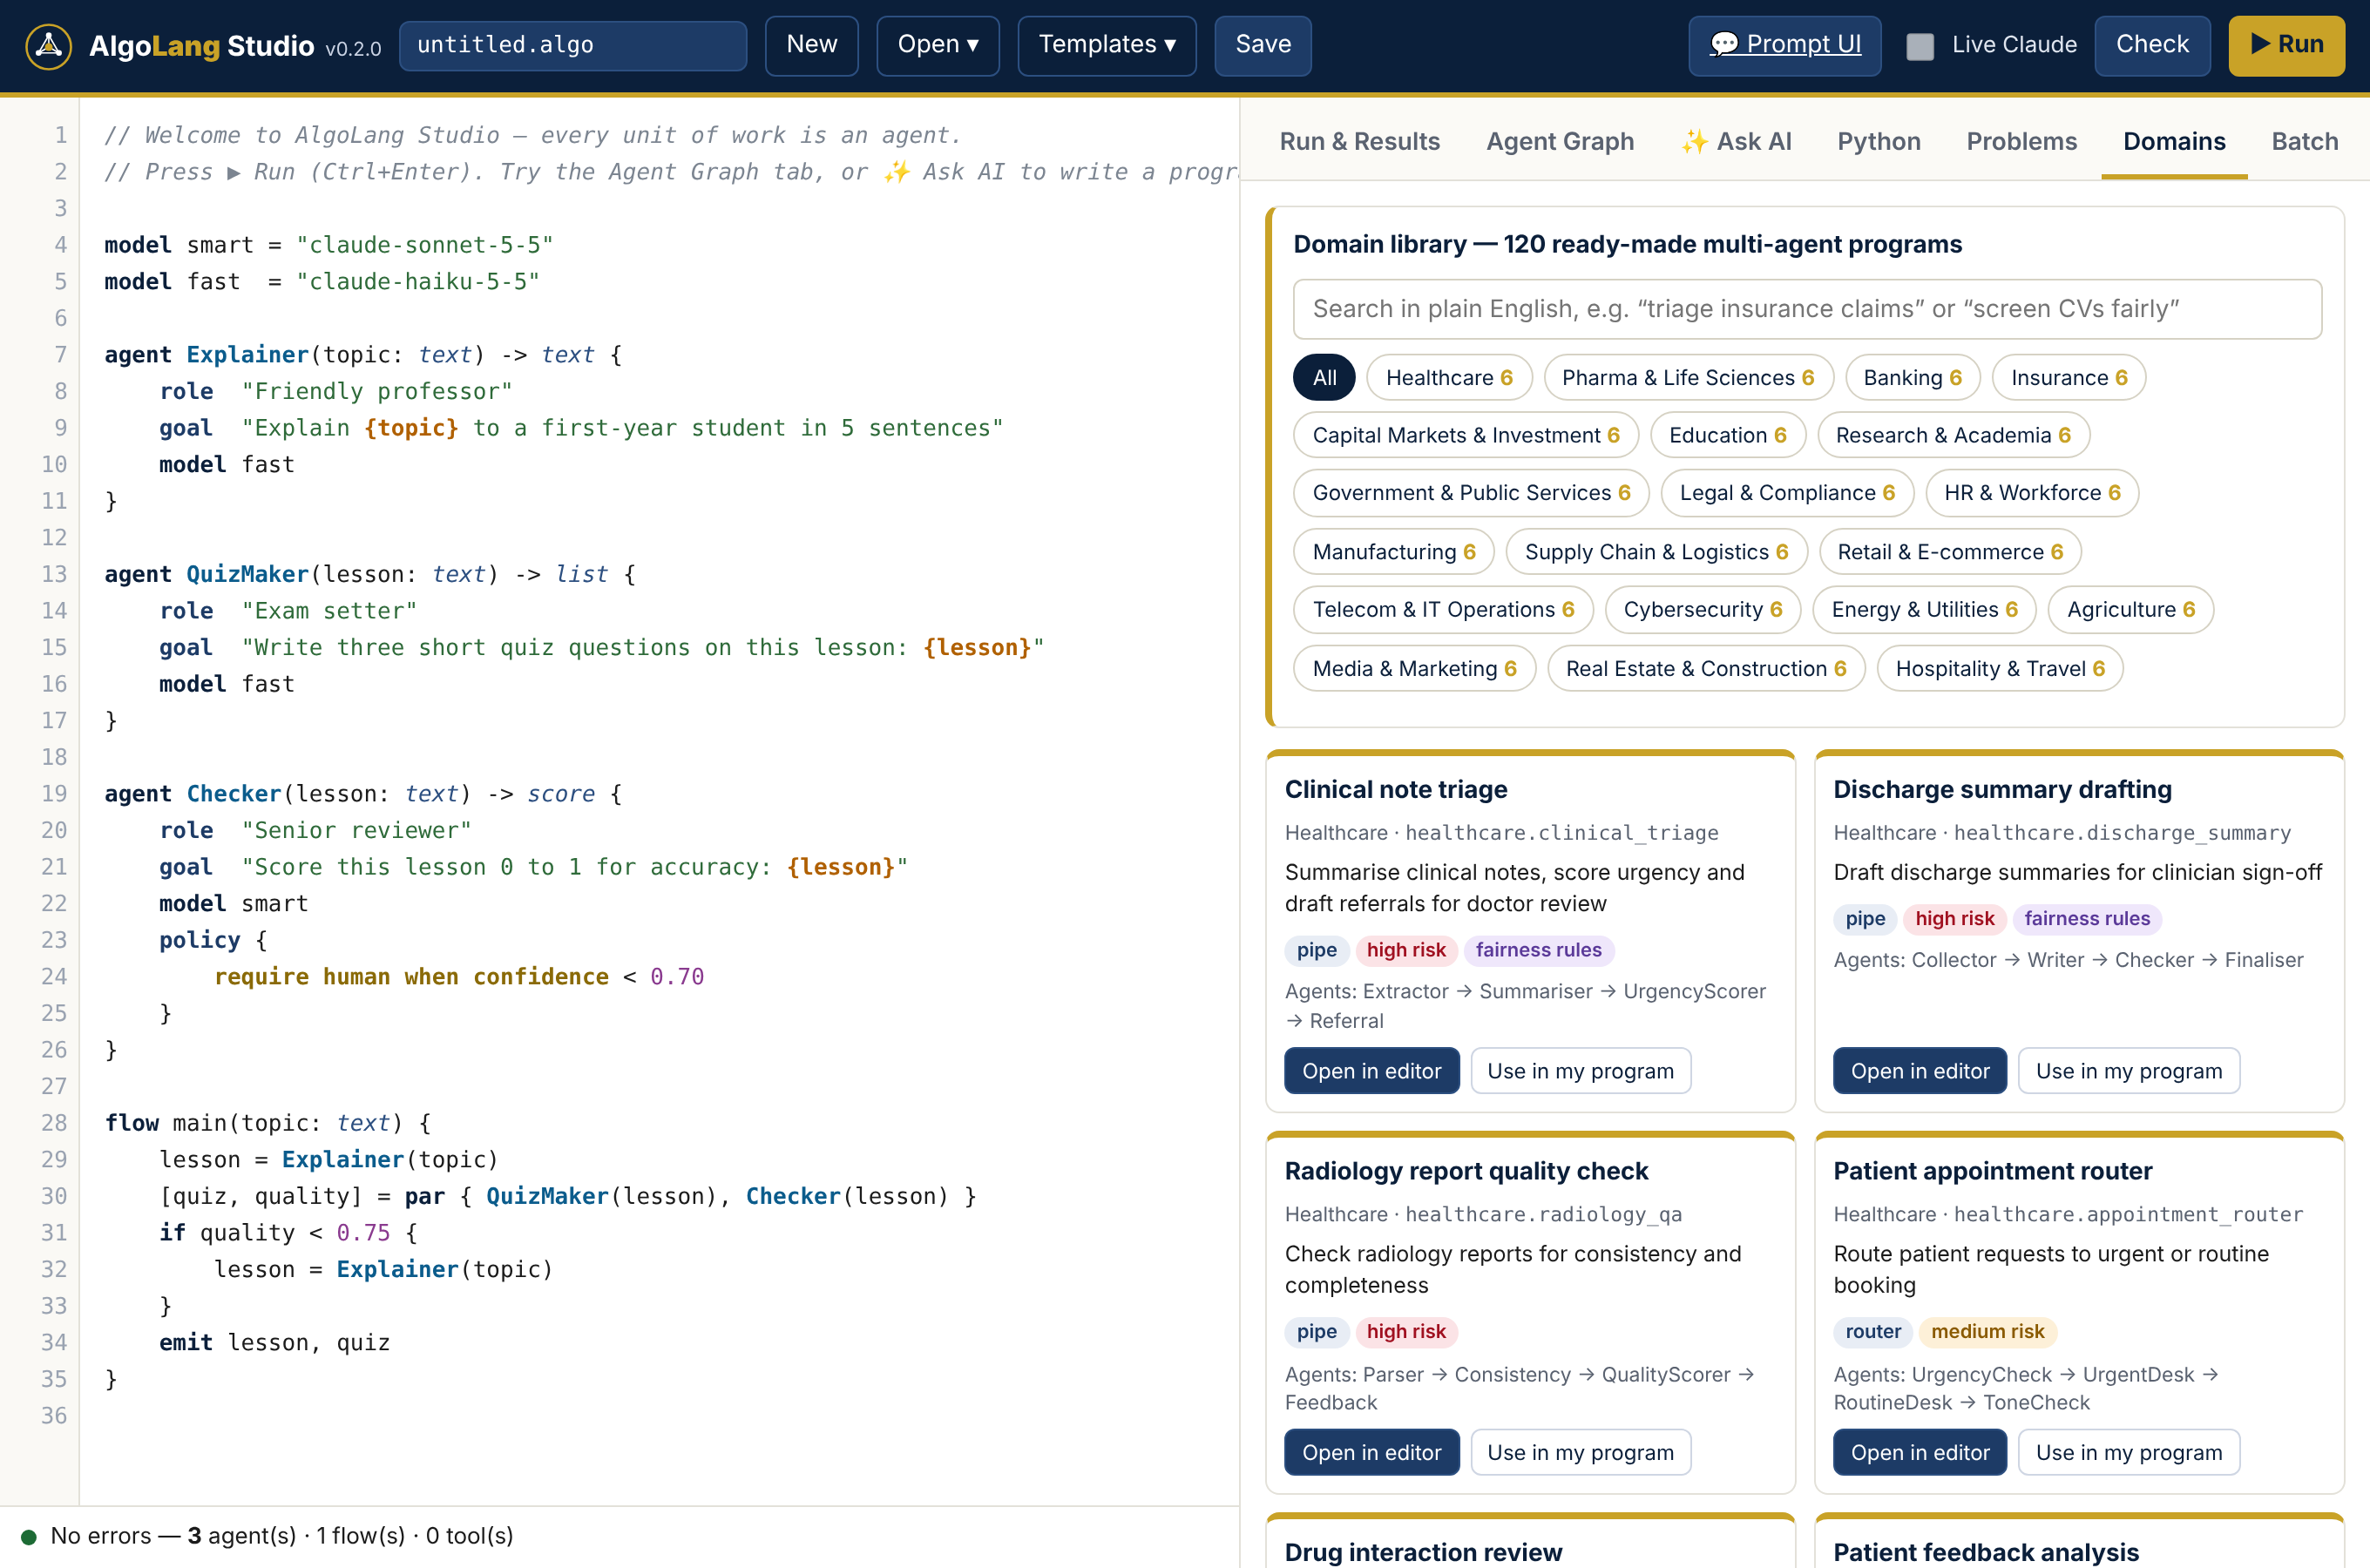
\includegraphics[width=\linewidth]{images/studio-domains.png}
\caption{Studio's Domains tab: 120 packs grouped by sector, each showing its pattern, risk level and agents.}
\label{fig:studiodomains}
\end{figure}

\begin{figure}[ht]
\centering
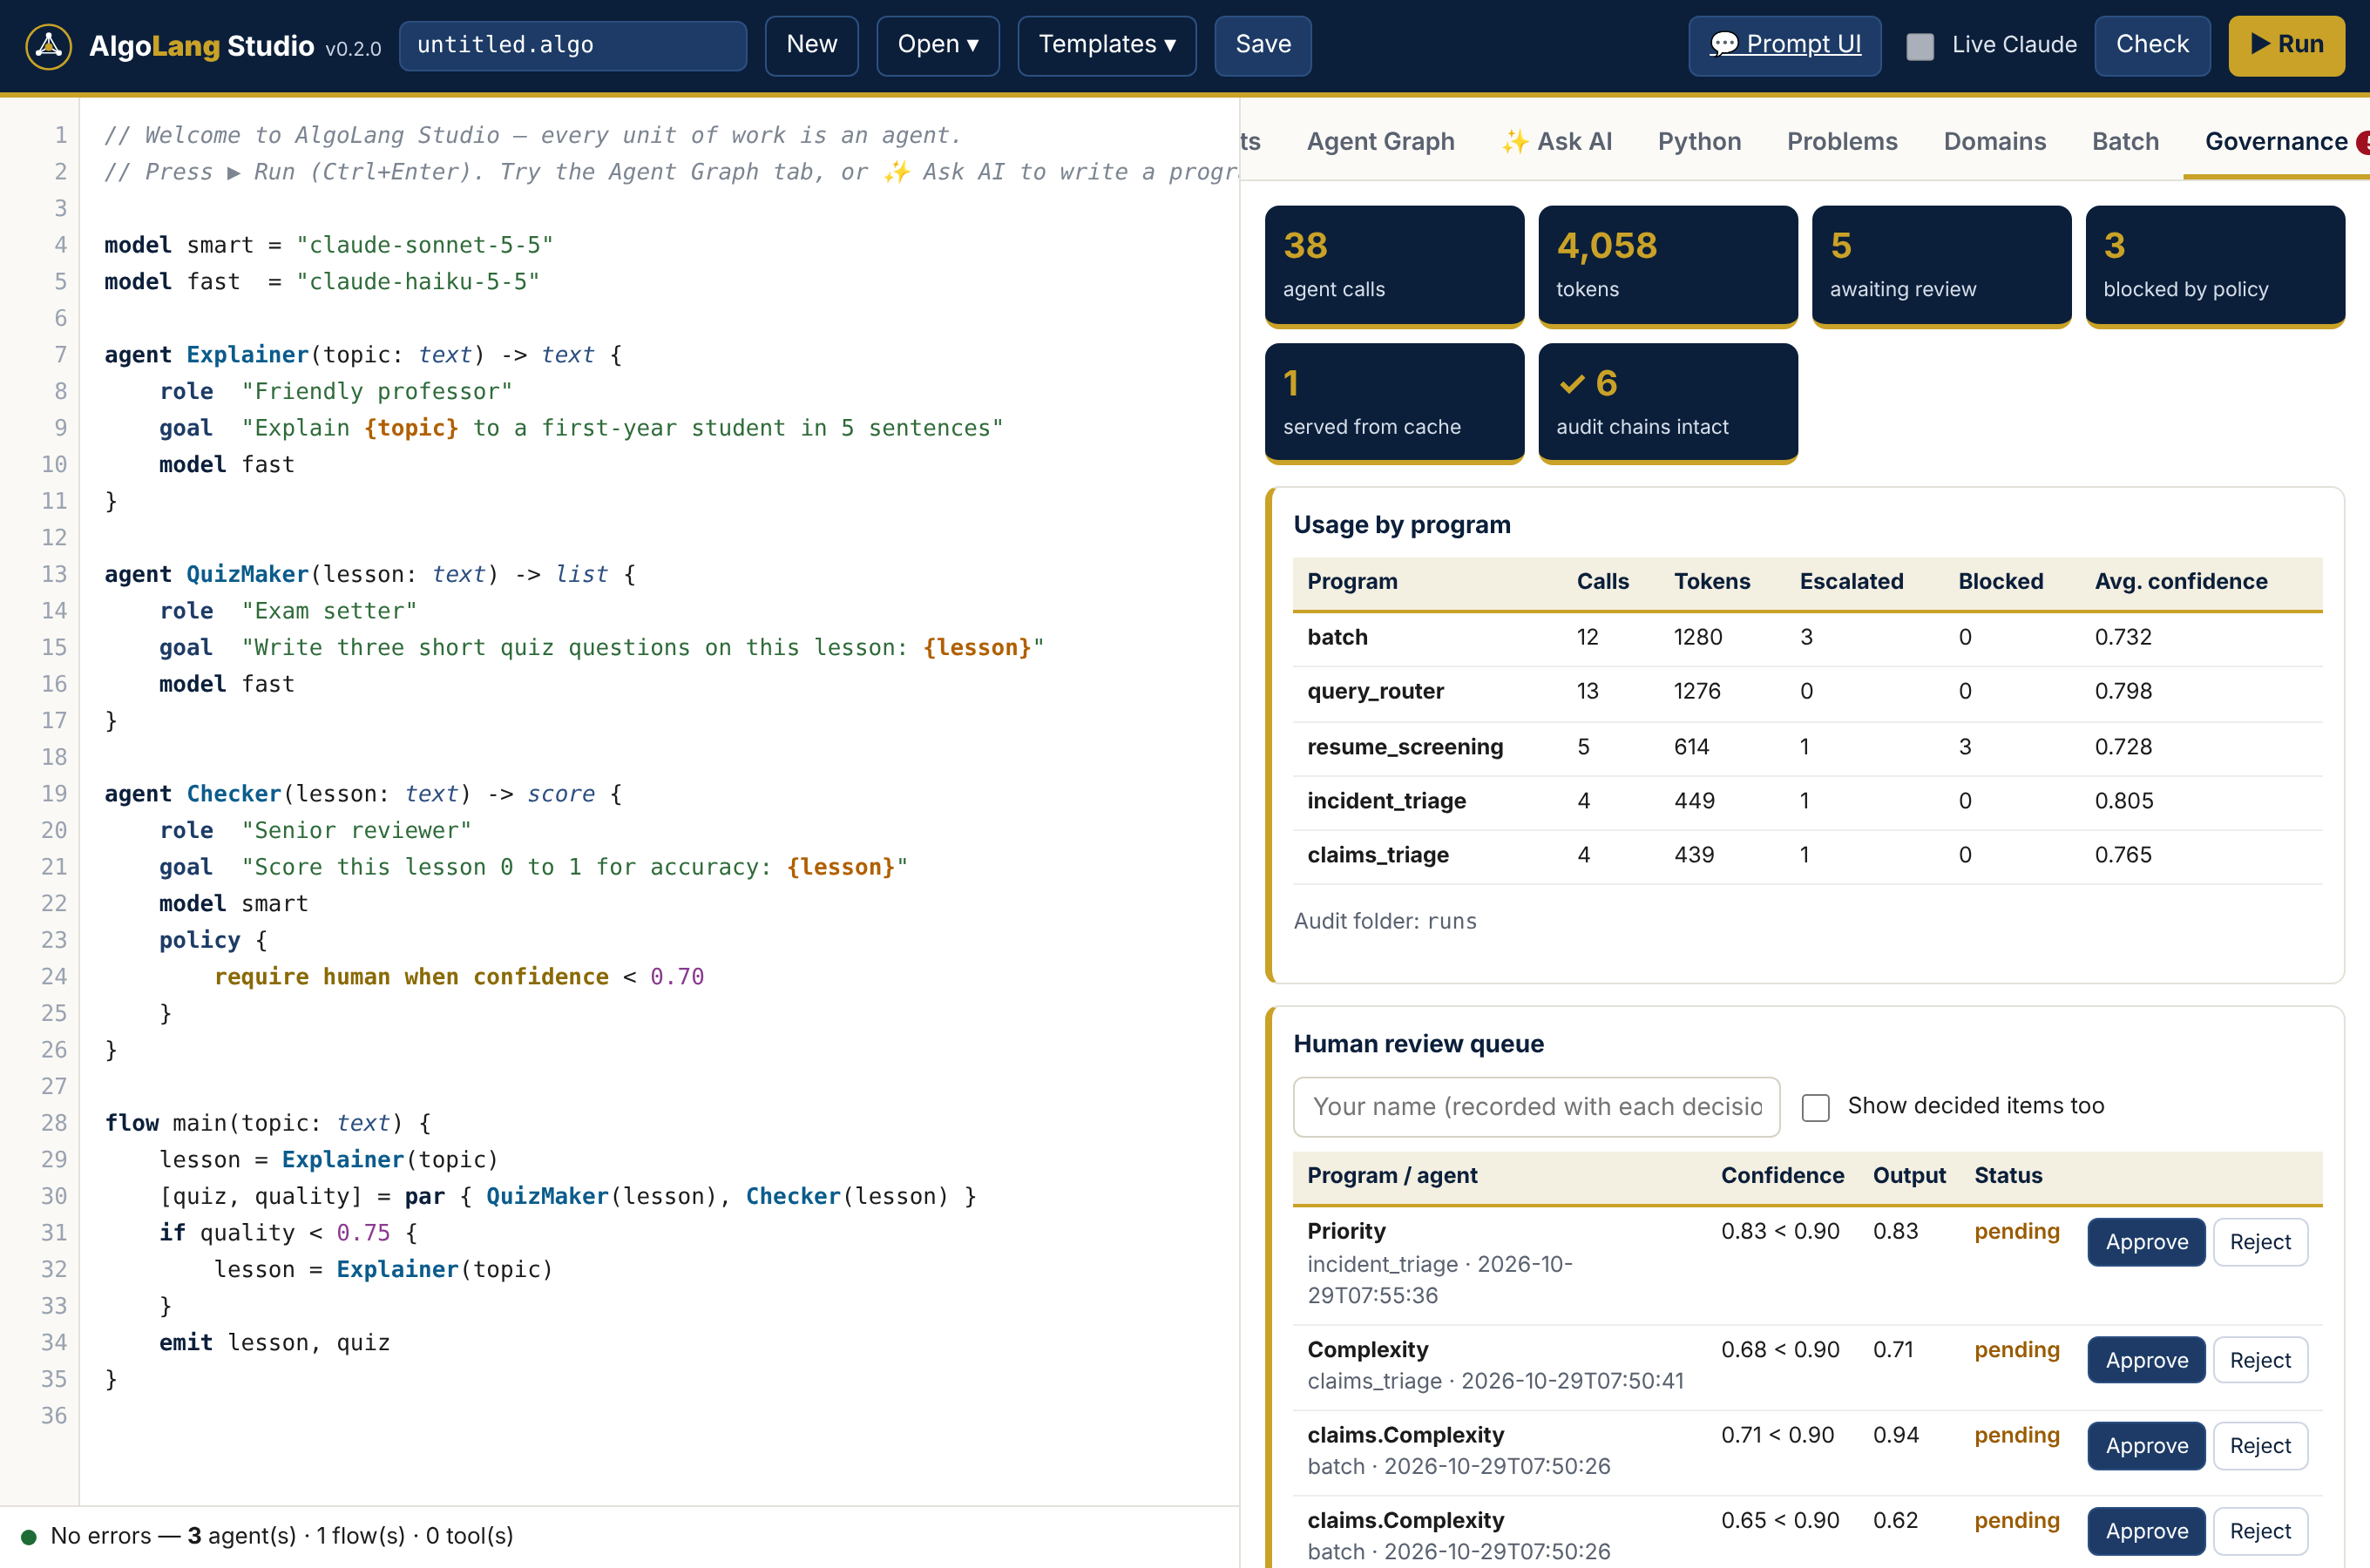
\includegraphics[width=\linewidth]{images/studio-governance.png}
\caption{Studio's Governance tab: usage and audit-chain tiles, usage per program, and the human review queue.}
\label{fig:studiogov}
\end{figure}

\subsection{Mode 3: Prompt-based UI}

\code{algo ui} opens a chat-style page for people who will never open an editor. They describe the problem in plain English. \algolang\ picks the best domain program, runs it under the org policy, and shows:
\begin{itemize}
\item the chain of agents;
\item the governance applied;
\item the result and any items waiting for human review;
\item a table of what each agent did;
\item the program source.
\end{itemize}
Alternatives are one click away. \emph{Open in Studio} hands the program to the graphical mode, and \emph{Customise with AI} asks Claude to adapt it (live mode).

\begin{figure}[ht]
\centering
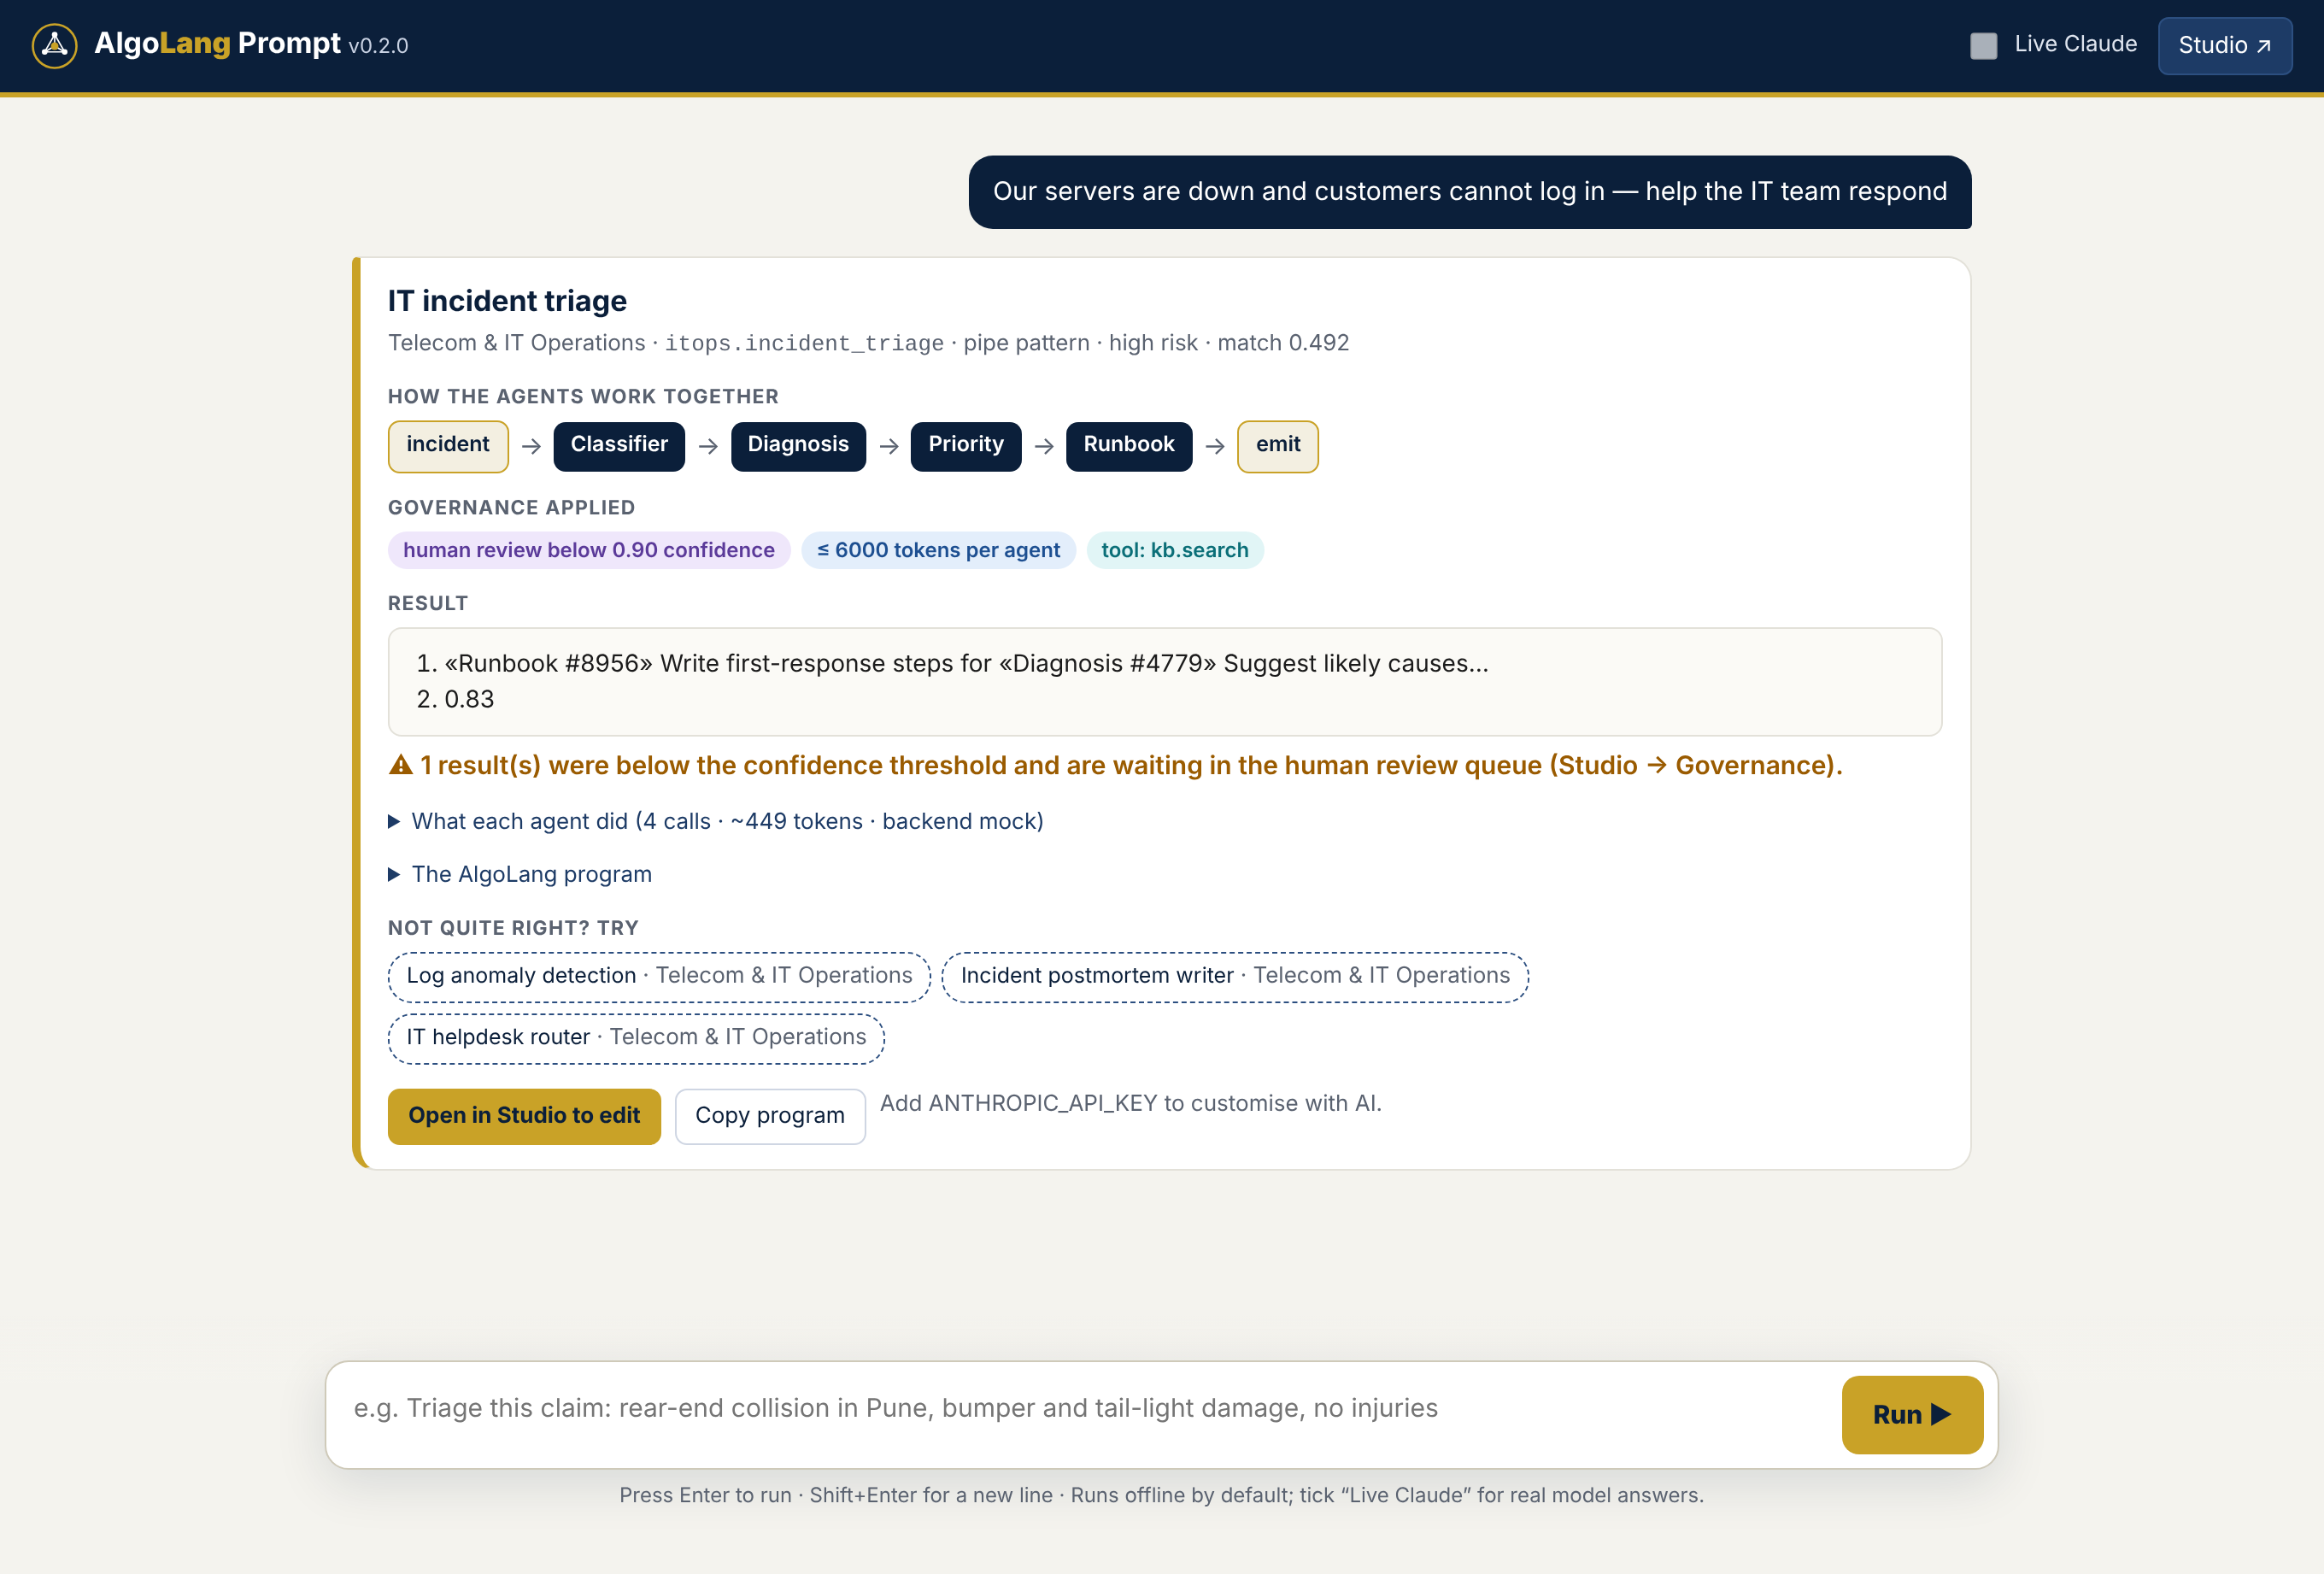
\includegraphics[width=\linewidth]{images/prompt-answer.png}
\caption{The Prompt UI answering an IT outage request with the \code{itops.incident\_triage} pack.}
\label{fig:promptui}
\end{figure}

\begin{ethics}
Governance in \algolang\ is enforced by the compiler and runtime. It is not left to good intentions. Forbidden attributes cannot reach an agent, low-confidence results wait for a named human, and any attempt to rewrite the audit trail is detected. Organisations should still review each domain pack before production use. The packs are well-governed starting points, not certified decision systems.
\end{ethics}
